% Fakesection 序言之前

\RequirePackage[l2tabu, orthodox]{nag}
\RequirePackage{ifxetex}
\RequireXeTeX

\documentclass{article}

%颜色
\usepackage{xcolor}

%长度
\usepackage{printlen}
\uselengthunit{mm}

%图形
\usepackage{pifont}
\usepackage{ean13isbn}
\usepackage{qrcode}
\usepackage{pdfpages}
\usepackage{overpic}
\usepackage{graphicx}
\graphicspath{{fig/}{img/}{etc/}}
\usepackage{media9}
\usepackage{wallpaper}
\usepackage{wrapfig}

%表格
\usepackage{tabu}
\usepackage{longtable}
\usepackage{booktabs}
\usepackage{diagbox}
\usepackage{multicol}
\usepackage{multirow}
\usepackage{makecell}
\usepackage{fancybox}
\usepackage{colortbl}
\usepackage{tcolorbox}
\tcbuselibrary{skins}
\tcbuselibrary{breakable}
\tcbuselibrary{theorems}
\tcbuselibrary{listings}
\tcbuselibrary{xparse}
\tcbuselibrary{minted}% 用minted排版代码
\usepackage{fvextra}
\usepackage{csvsimple}
\usepackage{boxedminipage2e}

%公式
\usepackage{amsmath}
\usepackage{amsthm}
\usepackage{amsfonts}
\usepackage{amssymb}
\usepackage{amsbsy}
\usepackage{amsopn}
\usepackage{amstext}
\usepackage{mathrsfs}
\usepackage{bm}
\usepackage{textcomp}
\usepackage{latexsym}
\usepackage{exscale}
\usepackage{relsize}
%\usepackage{xymtex}
\usepackage{physics}
\usepackage{siunitx}
\usepackage{hologo}
\usepackage{cases}

%文字
\usepackage{csquotes}
\usepackage{microtype}
\usepackage[heading=true]{ctex}
\setCJKfamilyfont{zhsong}[AutoFakeBold = {2.17}]{SimSun}
\renewcommand*{\songti}{\CJKfamily{zhsong}}

%正文
\usepackage{fancyhdr}
\usepackage{geometry}
\usepackage{lastpage}
\usepackage{indentfirst}
\usepackage{setspace}
\renewcommand\arraystretch{1}

%非正文
\usepackage{makeidx}
\makeindex
\usepackage{epigraph}
\usepackage{varwidth}
\usepackage{exercise}
\usepackage{tasks}
\renewcommand{\ExerciseName}{问题}
\renewcommand{\AnswerName}{回答}
\renewcommand{\listexercisename}{问题}

%参考文献
\usepackage{morewrites}
\renewcommand{\thefootnote}{\fnsymbol{footnote}}
\usepackage[resetlabels]{multibib}

%标题
\usepackage{caption}
\usepackage{subcaption}
\newcounter{sub}

%其它
\usepackage{atbegshi}
\usepackage{lipsum}

\csname
endofdump
\endcsname

%代码
\usepackage{minted}
\usepackage{boxie}
\makeatletter
\xdefinecolor{tcbcol@back}{rgb}{0,0,0}
\makeatother
\usepackage{tikz}
%%MatLab命令行
\newcommand{\MatlabLogo}{%
	\begin{tikzpicture}[x=2.4ex,y=2.4ex,line width=0ex,scale=1]
		\node[draw,fill=white,text=white] at (0, 0) (a) {
				\includegraphics[width=2.4ex]{matlabLogo.ai}
			};
	\end{tikzpicture}
}
\tcbset{%
	skin=enhanced,%
	matlab/.style={%
		skin=bicolor,%
		boxrule=0.1mm,%
		%toptitle=1ex,
		sharp corners,
		breakable,%
		colbacktitle=WinGray,%
		colframe=WinGray,%
		coltitle=black,%
		fonttitle=\sffamily,%\bfseries,
		fontupper=\small\sffamily,
		fontlower=\small\sffamily,
		frame style={%
			draw=WinBlue,%
			left color=WinBlue,%
			right color=WinBlue%
		},%
		overlay unbroken = {%
			\node[inner sep=0pt,anchor=north west,yshift=-3pt,xshift=1.2pt,text=black]
			at (frame.north west){\MatlabLogo};% \fbox{\faTerminal}
			\node[inner sep=0pt,anchor=north east,yshift=-3pt,xshift=-8pt,text=black] at (frame.north
			east){\rule{0.8em}{0.6pt}\quad$\square$\quad{\Large$\times$}};
		},%
		overlay first = {%
			\node[inner sep=0pt,anchor=north west,yshift=-3pt,xshift=1.0pt,text=black]
			at (frame.north west){\MatlabLogo};%\small ~\faWindows
			\node[inner sep=0pt,anchor=north east,yshift=-3pt,xshift=-8pt,text=black] at (frame.north
			east){\rule{0.8em}{0.6pt}\quad$\square$\quad{\Large$\times$}};
		}%
	},
	matlablight/.style={
		matlab,%
		colback=white,%
		colupper=black,%
		%coltext=black%
	},
	matlabdark/.style={
		matlab,%
		colback=black,%
		colupper=white,%
		%coltext=white%
	}
}
\DeclareTCBListing{matlabdarkc}{ m m }{%
	listing engine=minted,%
	minted style=trac,%
	minted options={%
		autogobble,%
		breaklines,%
		fontsize=\wuhao,%
		baselinestretch=0.6,%
		breaksymbolleft={},%
		numbersep=3mm%
	},%
	listing and comment,%
	colbacklower=tcbcol@back!5!yellow!10!white,%
	collower=linux,%
	matlabdark,%
	title={#2},%
	comment={\small\sffamily#1},%
	minted language=bat%
}
\DeclareTCBListing{matlablightc}{ m m }{%
	listing engine=minted,%
	minted style=trac,%
	minted options={%
		autogobble,%
		breaklines,%
		fontsize=\wuhao,%
		baselinestretch=0.6,%
		breaksymbolleft={},%
		numbersep=3mm%
	},%
	listing and comment,%
	colbacklower=tcbcol@back!5!yellow!10!white,%
	collower=linux,%
	matlablight,%
	title={#2},%
	comment={\small\sffamily#1},%
	minted language=bat%
}
\DeclareTCBListing{matlabdark}{ m }{%
	listing engine=minted,%
	minted style=trac,%
	minted options={%
		autogobble,%
		breaklines,%
		fontsize=\wuhao,%
		baselinestretch=0.6,%
		breaksymbolleft={},%
		numbersep=3mm%
	},%
	listing only,%
	matlabdark,%
	title={#1},%
	minted language=bat%
}
\DeclareTCBListing{matlablight}{ m }{%
	listing engine=minted,%
	minted style=trac,%
	minted options={%
		autogobble,%
		breaklines,%
		fontsize=\wuhao,%
		baselinestretch=0.6,%
		breaksymbolleft={},%
		numbersep=3mm%
	},%
	listing only,%
	matlablight,%
	title={#1},%
	minted language=bat%
}
\newtcbinputlisting{\matlabdarkcfile}[3]{%
	listing engine=minted,%
	minted style=trac,%
	minted options={%
		autogobble,%
		breaklines,%
		fontsize=\wuhao,%
		baselinestretch=0.6,%
		breaksymbolleft={},%
		numbersep=3mm%
	},%
	listing and comment,%
	colbacklower=tcbcol@back!5!yellow!10!white,%
	collower=linux,%
	matlabdark,%
	listing file={#3},
	title={#2},%
	comment={\small\sffamily#1},%
	minted language=bat%
}% end matlabdarkcfile
% 将文件做为窗口内容的Windows终端窗口样式命令
% 第1个参数是窗口底端提示信息
% 第2个参数是窗口标题
% 第3个参数是包含窗口内容的文件全路径名称(可以是相对路径)
\newtcbinputlisting{\matlablightcfile}[3]{%
	listing engine=minted,%
	minted style=trac,%
	minted options={%
		autogobble,%
		breaklines,%
		fontsize=\wuhao,%
		baselinestretch=0.6,%
		breaksymbolleft={},%
		numbersep=3mm%
	},%
	listing and comment,%
	colbacklower=tcbcol@back!5!yellow!10!white,%
	collower=linux,%
	matlablight,%
	listing file={#3},
	title={#2},%
	comment={\small\sffamily#1},%
	minted language=bat%
}% end matlablightcfile
% 将文件做为窗口内容的Windows终端窗口样式命令
% 第1个参数是窗口标题
% 第2个参数是包含窗口内容的文件全路径名称(可以是相对路径)
\newtcbinputlisting{\matlabdarkfile}[2]{%
	listing engine=minted,%
	minted style=trac,%
	minted options={%
		autogobble,%
		breaklines,%
		fontsize=\wuhao,%
		baselinestretch=0.6,%
		breaksymbolleft={},%
		numbersep=3mm%
	},%
	listing only,%
	matlabdark,%
	listing file={#2},
	title={#1},%
	minted language=bat%
}% end matlabdarkfile
% 将文件做为窗口内容的Windows终端窗口样式命令
% 第1个参数是窗口标题
% 第2个参数是包含窗口内容的文件全路径名称(可以是相对路径)
\newtcbinputlisting{\matlablightfile}[2]{%
	listing engine=minted,%
	minted style=trac,%
	minted options={%
		autogobble,%
		breaklines,%
		fontsize=\wuhao,%
		baselinestretch=0.6,%
		breaksymbolleft={},%
		numbersep=3mm%
	},%
	listing only,%
	matlablight,%
	listing file={#2},
	title={#1},%
	minted language=bat%
}% end matlablightfile

%链接%与beamer 冲突
\usepackage[
colorlinks = true,
linkcolor = gray,
citecolor = gray,
backref=page
]{hyperref}

%枚举%与beamer 干涉
\usepackage{enumitem}
\setlist[enumerate, 2]{
	fullwidth,
	label = \alph*.,
	font = \textup,
	itemindent = 2em
}

%标题%与beamer 冲突
\usepackage{titlesec}
\titleformat{\section}{\centering\LARGE\bfseries}{\thesection~}{0pt}{}

\begin{document}

% Fakesection 扉页

\begin{titlepage}
	\centering

	\includegraphics[width=.8\linewidth]{NJUST.ai}

	\vspace{10mm}

	\textbf{\heiti\zihao{0}电子信息工程}

	\textbf{\heiti\zihao{0}课程设计报告}

	\vspace{10mm}

	\begin{spacing}{2}

		\centering
		\zihao{2}

		\begin{tabu}to.8\linewidth{@{}X[4,r]@{}X[c]@{}X[12,l]@{}}
			\makebox[4\ccwd][s]{姓名} & :&\underline{\makebox[12\ccwd][c]{\kaishu 吴振宇 (916101630117)}}\\
			\makebox[4\ccwd][s]{}     & &\underline{\makebox[12\ccwd][c]{\kaishu 杨家钰 (9161040G1109)}}\\
			\makebox[4\ccwd][s]{学院} & :&\underline{\makebox[12\ccwd][c]{\kaishu 电子工程与光电技术学院}}\\
			\makebox[4\ccwd][s]{专业} & :&\underline{\makebox[12\ccwd][c]{\kaishu 电子信息工程}}\\
			\makebox[4\ccwd][s]{题目} & :&\underline{\makebox[12\ccwd][c]{\kaishu 心电信号的采集与分析}}\\
		\end{tabu}

		\vspace{0mm}%缩进

	\end{spacing}

	\zihao{2}\today

	\vspace{0mm}%缩进

\end{titlepage}

% Fakesection 摘要

\renewcommand{\abstractname}{\Large 摘要}
\begin{abstract}
	本课题设计利用信号发生器产生心电信号,然后运用DSP装置采集信号,之后用Matlab编程软件对信号进行处理。并且在原有的DSP程序上做了大量改进,将代码编译平台从已经过时的CCS3.3迁移到了CCS5向上兼容的所有版本,并增加了简单的GUI 图形显示功能。
\end{abstract}

\textbf{关键词:心电信号;DSP;Matlab。}

\newpage

%页眉页脚%与book冲突
\pagestyle{fancy}
\renewcommand{\headrulewidth}{0pt}
\lhead{\small{\leftmark}}
\chead{\small{\rightmark}}
\rhead{\small{第\thepage 页~共~\pageref{LastPage}~页}}
\lfoot{}
\cfoot{}
\rfoot{}

% Fakesection 目录

\pagenumbering{roman}

\tableofcontents
\listoffigures

\newpage

\pagenumbering{arabic}

\section{设计目的}%
\label{sec:设计目的}

心电信号属医学生物信号,一般具有以下特点:随机性较强,即信号无法用确定的函数来描述,而只是能用统计的方法,从大量测量结果中看其规律;噪声背景强,即要测的有用信号往往淹没在许多无用信号中。随着生活水平的提高,健康问题引起人们高度重视,在便携式自动心电诊断系统的项目背景下,便携式心电信号采集电路设计也越来越应用广泛。 \cite{彭飞武2007论心电信号检测中的噪声与干扰及其消除方法}

通过对心电信号的采集分析处理,可以有效地监测人的心脏和血压的健康状况。本次课程设计利用DSP实验装置首先采集心电传感器模块输出的心电信号,通过USB接口传输到计算机中,利用MATLAB编程对心电信号进行处理,显示出心电图波形,并对心电信号进行频谱分析。 \cite{江培海2016基于}

\section{设计要求}%
\label{sec:设计要求}

\begin{enumerate}
	\item 熟悉心电信号采集器的工作原理;
	\item 使用DSP实验箱进行心电波形数据采样,并通过USB将数据导入到计算机中以便进行分析;
	\item 使用MATLAB程序进行编程,显示已采样心电数据波形图,并经过隔直滤波后进行频谱分析;
	\item 通过查找资料,对心电图各项指标进行综合分析;再通过MATLAB编程测试这些指标并判断分析数据的正确性;
	\item 要求编程具有普遍性,即对所有数据适用,故要求采集两组不健康的情况进行对比试验。
\end{enumerate}

\section{设计步骤}%
\label{sec:设计步骤}

\subsection{MATLAB仿真}%
\label{sub:MATLAB仿真}

\begin{enumerate}
	\item 接通心电信号采集器以及传感器,连接到示波器,利用信号发生器产生心电信号,利用示波器测量确认后,通过连接电缆将心电信号采集器或者信号发生器的输出连接到的C2000DSP实验箱的INPUT1端口。
	\item 将DSP实验箱的OUT3端口连接示波器。
	\item 接通DSP实验箱电源,根据液晶显示屏显示的提示信息进行操作。
		\begin{enumerate}
			\item 上电后,首先选择4(AD),按ENTER键确认;
			\item 通过数字键选择采样频率(符合那奎斯特采样定理,本次试验中采用300Hz),按 ENTER 键确认;
			\item 选择“1”保存,通过主机上的采集软件,可将采集的数据通过 USB 线上传到主机。选则“2”不保存,可通过 DSP 试验箱的 OUT3 接口,通过示波器观察波形,若系统正常,应该能够看到跟信号发生器输出一致的波形,以此来验证电路系统的正确性;
			\item 若在 3)选择“1”保存后,主机会提示安装USB驱动,正确安装驱动后,打开主机上的数据采集软件,会出现如图所示界面:
			\item 点击“start”,开始数据传输,若系统工作正常,Successed Transfers 后会显示“5”,表明收到5个数据包,若显示信息不是5,则将 DSP 试验箱断电,重新开始。
			\item 若5)正常,则主机会产生一个数据文件 USB.DAT,这就是ADC采集的数据,共 1024个采样点,每个采样点为12位有效数字,表示为2个字节,高8位在前(其中高4位为 0),低8位在后。
		\end{enumerate}
	\item 在PC端接收实验箱传输的采样数据,利用编好的MATLAB程序进行数据处理。
	\item 观察PC端MATLAB显示结果,逐步调试改进程序。
	\item 修改程序并对数据进行分析最后给出健康分析。
	\item 重新采集三组数据进行对比试验。三组信号分别为:
		\begin{enumerate}
			\item 0.8Hz,300Mv
			\item 1Hz,400mV
			\item 2Hz,600mV
		\end{enumerate}
\end{enumerate}

心电信号的分析参照一下标准:

\begin{figure}[H]
	\centering
	\includegraphics[width=0.8\linewidth]{standard.png}
	\caption{正常心电图波形示意图}
	\label{fig:正常心电图波形示意图}
\end{figure}

心电图的各个指标正常要求范围如下:

\begin{enumerate}
	\item PR间期:(120~200)ms。
	\item QRS宽度:(60~100)ms。
	\item QT间期:(340~430)ms(跟心率很相关,此为对应60~100bpm的QT间期正常最高值)。
	\item $ \mathrm{QT}_\mathrm{C} $间期:< 440ms ($ \mathrm{QT}_\mathrm{C}= \dfrac{QT}{\sqrt{RR}} $为心率校正的QT间期,临界$ \mathrm{QT}_\mathrm{C} $值为440~460ms,>460ms判断为QT延长,<350ms为缩短)。
	\item ST段:(-0.05~0.3)mV,(超过正常范围下移常见于心肌缺血或劳损,上移多见于急性心肌梗塞、急性心包炎等)。
	\item P波幅度$ \leqslant $0.25mV ,宽度$ \leqslant $0.11s。
	\item Q波幅度同导联1/4R波振幅宽度$ \leqslant $0.04s。
	\item QRS波群较复杂,一般可认为(0.5~2.0)mV。
	\item T波幅度$ \geqslant $同导联1/10R波幅度,胸前导联T波幅度高达(1.2~1.5)mV,T波低平或者倒置常见于心肌缺血、低血钾等。
	\item U波:振幅很小,在胸前导联特别是V3较清楚,可高达(0.2~0.3)mV。
	\item 正常窦性心率(60~100)bpm (对应的RR间期为(1~0.6)s)。
\end{enumerate}

MATLAB程序编写以及数据分析原理:

\begin{enumerate}
	\item 实验数据在通过DSP实验箱进行数据采集时会产生电噪声,影响数据分析,故在数据频谱分析前需要进行隔直、归一化与滤波,实验中滤除直流分量可以使用参考语句 ,滤波采用加凯瑟窗(具体程序见附录二)。
	\item 心率即心脏在一分钟之内跳动的次数,其产生次数表现在波形上即为一段时间内R峰出现的次数,因而计算心率即要求使用MATLAB编程在处理过的数据中找到所有最大波峰(使用findpeak()函数),给出所有最大波峰的横纵坐标即时间和电压,对相邻波峰出现的时间间隔取平均数$ t $,使用公式:心率$ = \dfrac{60}{t} $
	\item Q/S点的查找,首先规定一定阈值,在这个阈内,Q/S点即为最大或者最小点,此时使用函数max()即可得到相应的横纵坐标;
	\item Q波、T波和S波的脉冲宽度,这三个波可以视为正弦波的部分,通过在一定范围内,当数值开始出现连续性的变化时,可以视为这个开始产生变化的点即为以上各波的起始点,它们与波峰或者波谷点的横坐标差的二倍即为波的时间宽度,进行转化,得到脉冲宽度。
	\item 血压的高低与心率的大小成正比;
	\item 健康分析综合各项指标进行。
\end{enumerate}

\subsection{DSP开发}%
\label{sub:DSP开发}

\begin{figure}[H]
	\centering
	\includegraphics[width=0.3\linewidth]{dia.pdf}
	\caption{流程图}
	\label{fig:流程图}
\end{figure}

现有的DSP例程存在如下问题:

\begin{enumerate}
	\item 该例程运行于CCS3.3 ,平台版本过老,编译器已经过了TI公司的支持期,不再维护;
	\item 该例程采用字模,显示较为麻烦;
	\item 该例程未能充分利用LCD 的功能,没有提供GUI 图形显示的API。
\end{enumerate}

针对如上问题,先将程序迁移到了CCS5 ,删除了编译器已经提供的静态链接库,减少了程序的冗余; 在修改了文件包含路径、静态链接库搜索路径等工程变量后,程序可以成功编译并烧录。

然后对程序进行重构,因为没有硬件原理图的缘故,不知道芯片内部连线,避开了对底层寄存器的修改。主要重构的部分在LCD的显示上,修改了原先显示的API,使得可以支持图片的显示。函数允许在指定的坐标显示指定大小的点阵图片。

最后修改了算法的部分逻辑,当计算出结果后直接在屏幕上显示。

\section{设计结果}%
\label{sec:设计结果}

\subsection{MATLAB仿真结果}%
\label{sub:MATLAB仿真结果}

\begin{figure}[H]
	\centering
	\begin{subfigure}[H]{.45\linewidth}
		\centering
		\includegraphics[width=\linewidth]{arb1.png}
		\caption{量化后的心电图}
		\label{fig:量化后的心电图}
	\end{subfigure}
	\quad
	\begin{subfigure}[H]{.45\linewidth}
		\centering
		\includegraphics[width=\linewidth]{arb2.png}
		\caption{加窗后的心电图}
		\label{fig:加窗后的心电图}
	\end{subfigure}
	\caption{MATLAB仿真图}
	\label{fig:MATLAB仿真图}
\end{figure}

\begin{figure}[htpb]
	\centering
	\matlablightfile{MATLAB Command Window}{txt/arb.txt}
	\caption{运行界面}
	\label{fig:运行界面}
\end{figure}

\subsection{DSP开发结果}%
\label{sub:DSP开发结果}

\begin{figure}[H]
	\centering
	\begin{subfigure}[H]{.3\linewidth}
		\centering
		\includegraphics[width=\linewidth]{step1.jpg}
		\caption{第一步}
		\label{fig:第一步}
	\end{subfigure}
	\quad
	\begin{subfigure}[H]{.3\linewidth}
		\centering
		\includegraphics[width=\linewidth]{step2.jpg}
		\caption{第二步}
		\label{fig:第二步}
	\end{subfigure}
	\quad
	\begin{subfigure}[H]{.3\linewidth}
		\centering
		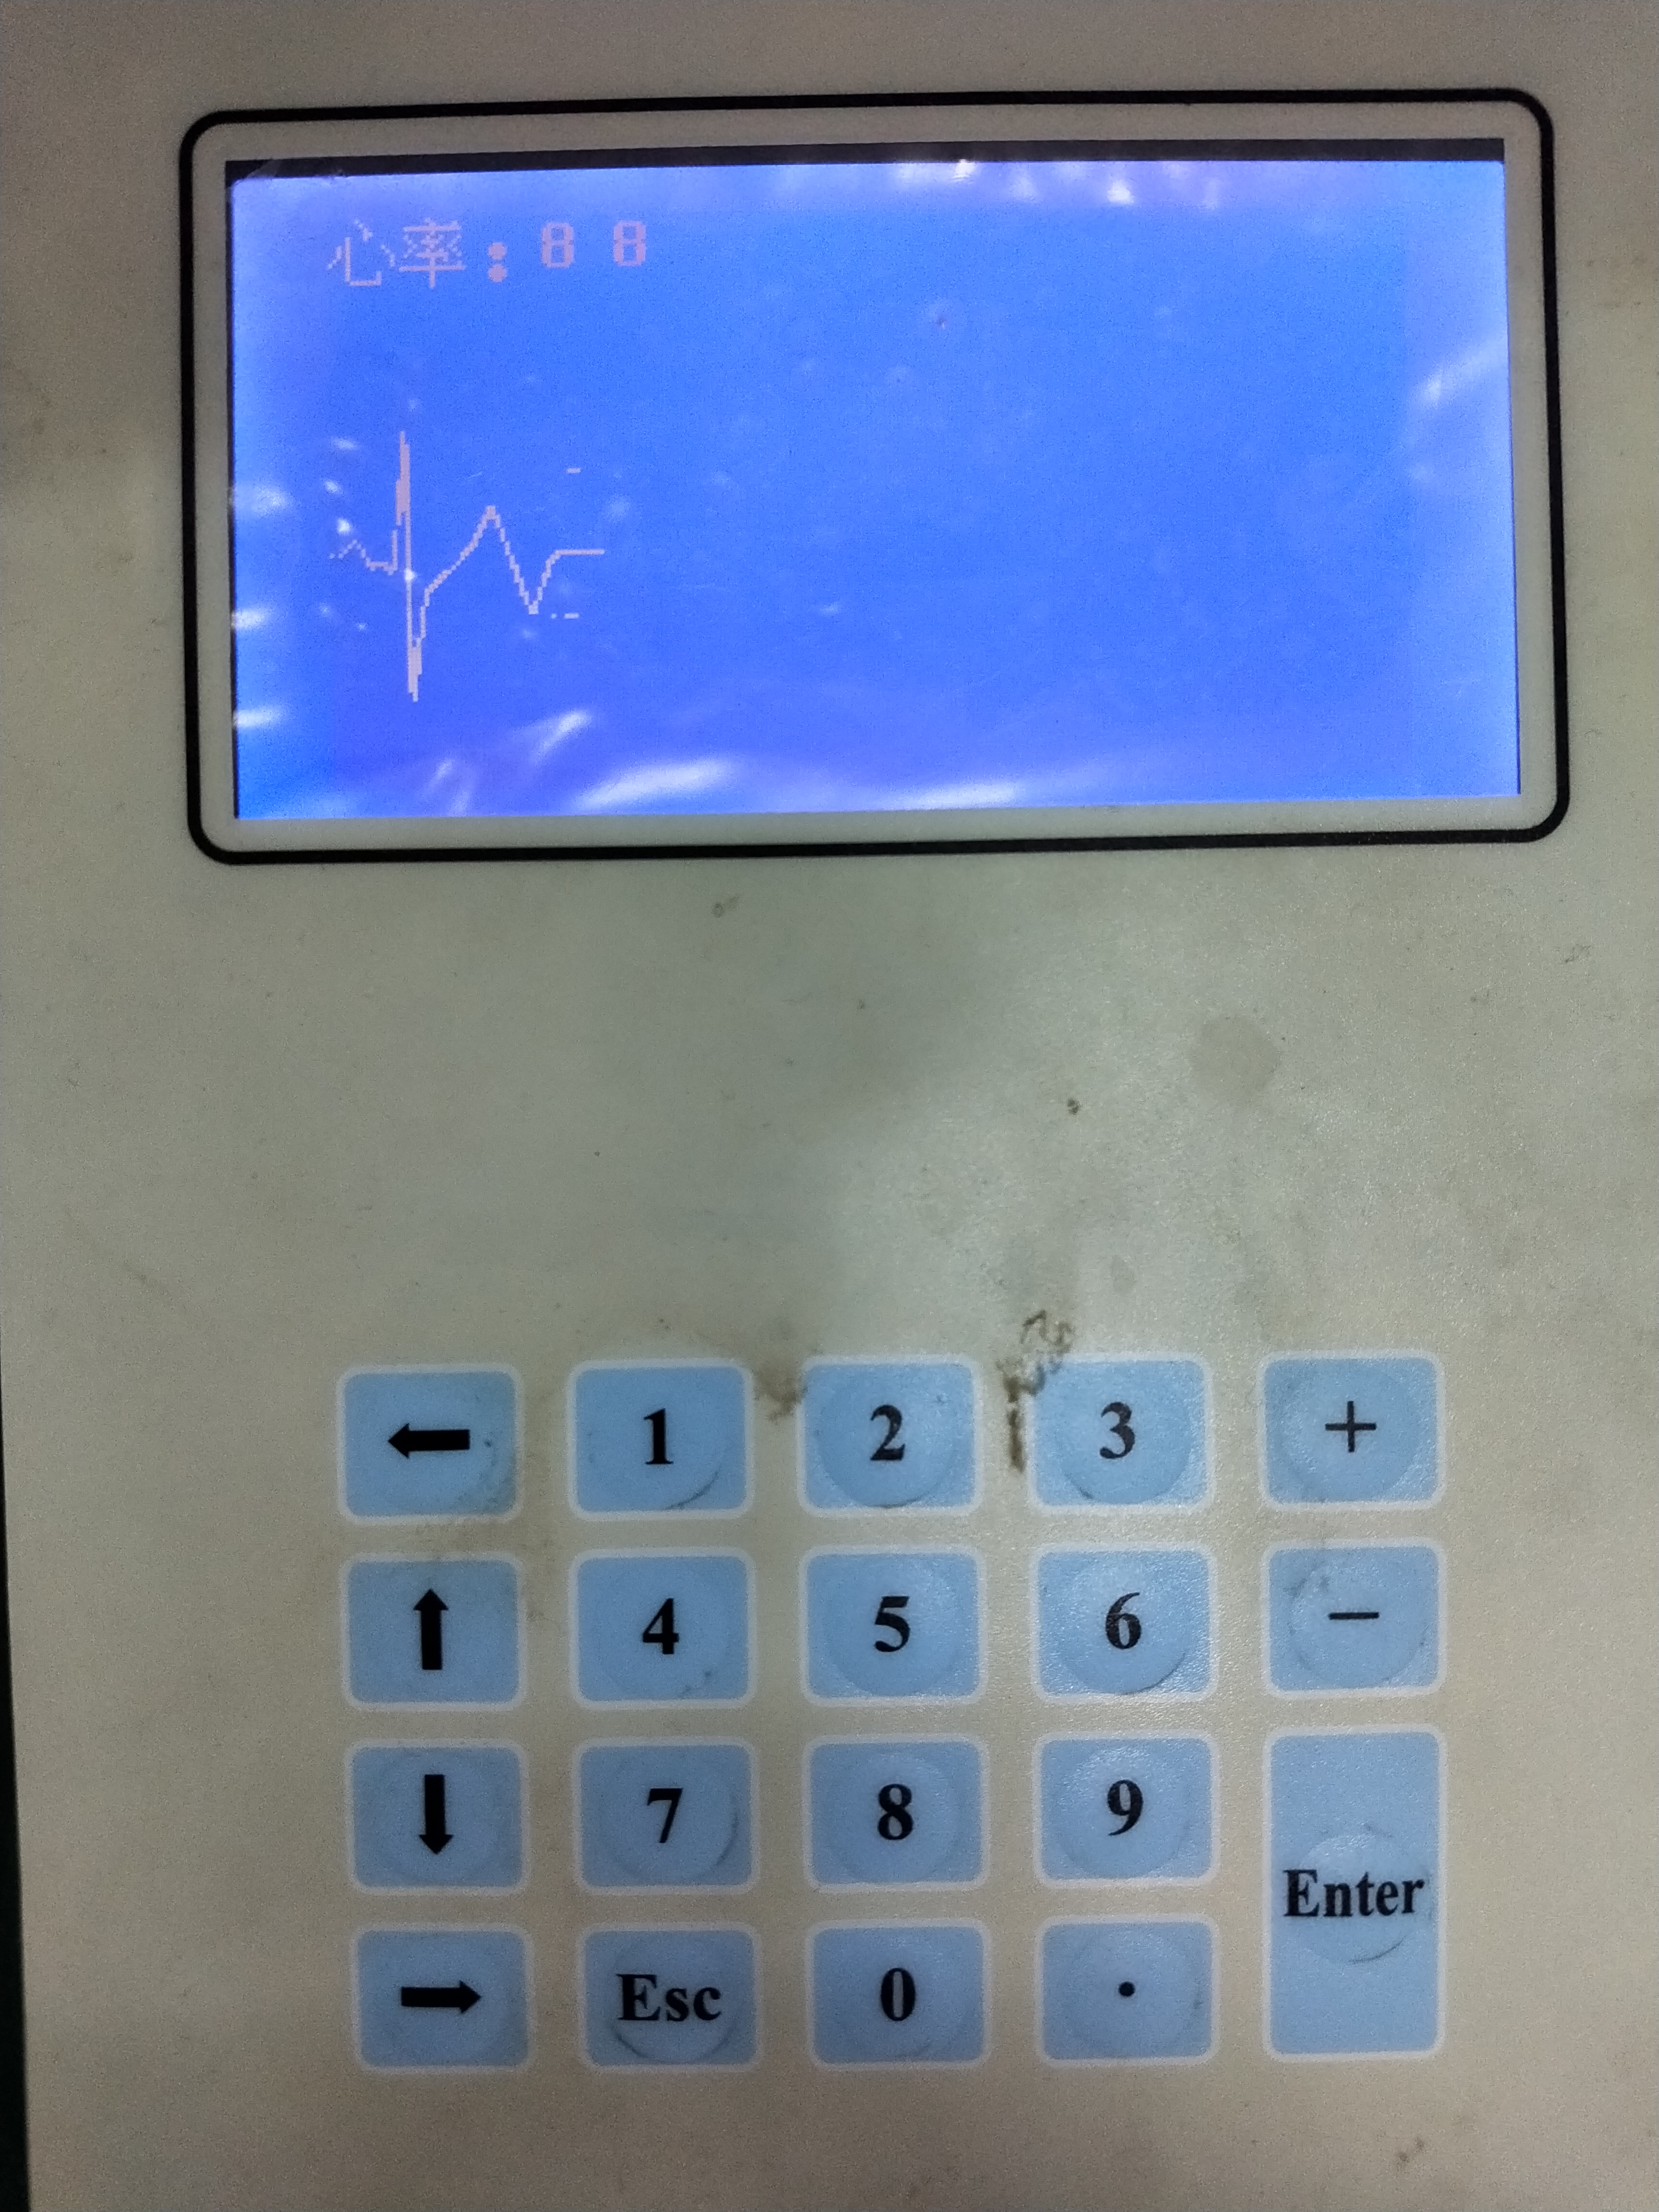
\includegraphics[width=\linewidth]{step3.jpg}
		\caption{第三步}
		\label{fig:第三步}
	\end{subfigure}
	\caption{运行结果}
	\label{fig:运行结果}
\end{figure}

\section{设计总结与心得体会}%
\label{sec:设计总结与心得体会}

本次课程设计利用信号发生器产生心电信号,然后运用DSP采集信号,之后用Matlab编程软件对信号进行处理。

本次课程设计学习了CCS软件的功能和用法,加深了对MATLAB软件的了解。学会了信号的采集与分析。掌握了简单心电信号采集与分析的电路和原理,通过实践提高了综合能力。

% Fakesection 参考文献

\bibliographystyle{IEEEtran}
\bibliography{bib/main}

% Fakesection 附录

\renewcommand{\thesection}{\Alph{section}~}

\appendix

\section{代码}%
\label{sec:代码}

\subsection{MATLAB仿真重要代码}%
\label{sub:Matlab仿真重要代码}

\langCVfile[Matlab][lst:arb.m][Matlab]{arb.m}{\string"lst/arb.m\string"}

\subsection{DSP开发重要代码}%
\label{sub:DSP开发重要代码}

\langCVfile[c][lst:test.c][c]{test.c}{\string"lst/test.c\string"}

% Fakesection 索引

\printindex

\end{document}

